\chapter{Revisão Bibliográfica}

A modelagem de robôs de acordo com suas principais funcionalidades e o
desenvolvimento de novas arquiteturas são o âmago no estudo de
controle de missão de robôs móveis. Dessa forma, arquitetura robótica e controle
de missão são conceitos relacionados, e, portanto, o cerne desta pesquisa
bibliográfica. 

Neste capítulo, são apresentados os fundamentos teóricos necessários para o
entendimento desta dissertação. O objetivo deste levantamento bibliográfico é
apresentar alguns dos principais trabalhos e pesquisas científicos sobre
arquiteturas e sistemas de controle de missão de robôs móveis. Por fim,
o leitor é direcionado para os conhecimentos aplicados no controle de missão do
robô DORIS, projeto que envolve esta dissertação.

O conceito de arquitetura %do grego arkhétékhton, do ingles architecture, do
% frances architecture
 para robôs é definido de diferentes formas na
literatura. Em \cite{arkin1998behavior}, arquitetura de robô é
relacionada com arquitetura de software, em uma adaptação à
arquitetura de computadores de \cite{stone1980introduction}, e definida como:
arquitetura de robô é a disciplina dedicada ao projeto de robôs altamente específicos e individuais
a partir de uma coleção de blocos comuns de softwares.
Em \cite{mataric1992behavior}, a definição aborda sistemas de controle: uma
arquitetura fornece uma maneira principal de organizar um
sistema de controle, contudo, a arquitetura também impõe restrições sobre a
forma como o problema de controle pode ser resolvido. Já
em \cite{brooks1986robust}, o autor tenta associar a arquitetura de software
com os componentes de hardware (processadores) para compor a arquitetura
robótica.

O sistema robótico é composto por diversos elementos de hardware e
software que são interdependentes e necessários para o funcionamento do sistema.
Como o propósito deste trabalho é o desenvolvimento de uma arquitetura robótica
para o DORIS, sendo considerados os aspectos físicos, lógicos e a aplicabilidade do
robô, entende-se que uma arquitetura para robô móvel descreve uma maneira de se construir o
controle inteligente do robô, os módulos do sistema, como estes
módulos interagem entre si e seus elementos de hardware associados, visando sua
aplicação. A evolução das arquiteturas apresentadas nesta revisão
bibliográfica mostra que os elementos de hardware assumem um papel de grande
importância durante o desenvolvimento dessas arquiteturas, por exemplo como um
fator limitador, assim como a aplicação e o meio em que o robô está inserido.

De acordo com \cite{siegwart2004autonomous}, os componentes básicos de uma
arquitetura para robôs são classificados em três grupos: \textit{Percepção}, que
envolve as atividades de interpretação e integração dos sensores;
\textit{Planejamento} de tarefas, sincronização,
e o monitoramento da execução de todas as atividades do robô; \textit{Atuação},
que envolve as atividades de execução dos movimentos, ações do robô e controle
dos atuadores.

As três primeiras seções desta pesquisa bibliográfica abordam os paradigmas da
robótica, isto é, as três arquiteturas de operação de um sistema robótico:
paradigma hierárquico/deliberativo (SPA - \emph{Sense, Plan and Act}); paradigma
reativo; e paradigmo híbrido deliberativo/reativo. As seções apresentam e
exemplificam as arquiteturas pela ótica de diversos autores, e são
comparadas e analisadas.

%TODO: acrescentar mais uma referência (arkin?)
O controle de missão ou planejamento de missão de robôs faz parte da arquitetura
robótica, e pode ser desenvolvido para os três tipos de arquiteturas. Em
\cite{fryxell1996navigation}, é apresentada uma das primeiras definições de
controle de missão para robôs: controle de missão é um sistema que permite ao
operador definir as missões de um veículo em linguagem de alto nível; provê
ferramentas adequadas para converter planos em Progamas de Missões que podem
ser verificados e executados em tempo real; e permite ao operador saber o
estado da missão enquanto esta é executada, e modificá-la se for necessário. Em
\cite{brumitt1996dynamic}, o conceito de planejamento de missão é ampliado para
múltiplos robôs: planejamento de missão é o processo de determinar o
que cada robô deve fazer para alcançar os objetivos da missão, em um ambiente
dinâmico. 

Neste trabalho, o controle de missão de robôs é o componente da arquitetura
robótica que organiza e executa todas as tarefas do robô de maneira ótima,
exerce o papel de traduzir os comandos de missão do usuário ao robô, provê feedback ao
operador, e contém as diretivas do robô. Como faz parte da arquitetura, as
seções que seguem buscam, em cada arquitetura, destacar de forma exemplificada
alguns controles de missão.

\section{Paradigma hierárquico/deliberativa}
Em meados do século XX, são realizados os primeiros estudos de robôs autônomos,
juntamente com o aparecimento da Inteligência Artificial (IA). Em um sistema
robótico, a IA clássica consiste em um modelo centralizado que coleta
informações usando sensores, cria um modelo do ambiente, planeja o próximo
movimento e executa a ação. São sistemas do tipo \emph{Sense, Plan and
act} (SPA). Essa arquitetura de controle é clássica e tem abordagem
\emph{top-down} (hierárquica), como na decomposição tradicional da
figura~\ref{BROOKS_1}.
%TODO: Mudar essa figura

De acordo com Marvin Minsky, uma máquina deveria tender a criar, por si só, um
modelo abstrato do ambiente em que está inserido (defina-se \emph{mundo}).
Caso fosse dado uma tarefa, ela primeiro poderia explorar soluções dentro de seu modelo abstrato e, então,
experimentá-las externamente. Seria como realizar uma simulação interna
e, caso funcionasse, realizá-la no mundo real.

\subsection{Robôs deliberativos}
Entre 1966 e 1972, Charles Rosen e Nils Nisson da Universidade de Stanford
criaram o Shakey, primeiro robô móvel autônomo (figura~\ref{SHAKEY_1}). Foi
desenvolvida uma inteligência artificial, \textit{problem solver}, chamada
STRIPS. Este sistema é um planejador de trajetórias que armazena as imformações
do ambiente (mapas e obstáculos) de maneira simbólica e, se dada uma tarefa de
deslocamento (\textit{goto}), é realizada uma busca lógica pelo sistema.

Em 1977, começou a ser desenvolvido o projeto HILARE (figura~\ref{hilare}), no
Laboratoire d'Automatique et d'Analyse des Systèmes (LAAS), Toulouse, France. Possuía sensores como câmera, quatorze ultrassons e laser para
medir distância, sendo possível atualizar o seu mundo com acurácia. Seu mundo
era representado por modelos geométricos e um modelo relacional que expressava a
conectividade dos quartos e corredores (simbólico) \cite{norelis1989control}.

Também em 1977, o Stanford Cart foi criado por Moravec para teste de visão
para navegação e desvio de obstáculos \cite{moravec1977towards}. Os obstáculos
eram identificados pelo robô durante a operação e representados em seu mundo
como esferas. O mundo também era representado simbolicamente por grafos.

Em 1969, Victor Scheinman, Universidade de Stanford
\cite{scheinman1969design}, inventou o primeiro manipulador robótico
totalmente elétrico de seis elos e com solução completa e integrada de
cinemática inversa. Isto é, dado um ponto qualquer pertencente ao espaço de
trabalho do manipulador, este calcula o ângulo das juntas de forma que o
efetuador alcance o ponto especificado. Isso permitiu que o manipulador
percorresse trajetórias arbitrárias. Até os dias atuais, 2015, é ampla a
utilização de manipuladores industriais. A sofisticação destes sistemas já
possibilita que estes armazenem todo o conhecimento do mundo e executem tarefas
autônomas (figura~\ref{manipulador}).

\begin{figure}[H]
\centering
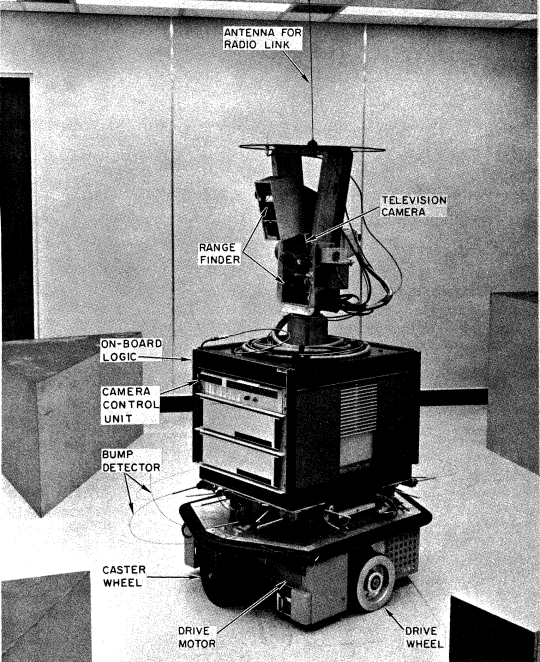
\includegraphics[width=1\columnwidth]{figs/SHAKEY_1.png}
\caption{Shakey robot}
\label{SHAKEY_1}
\end{figure}

\begin{figure}[H]
\centering
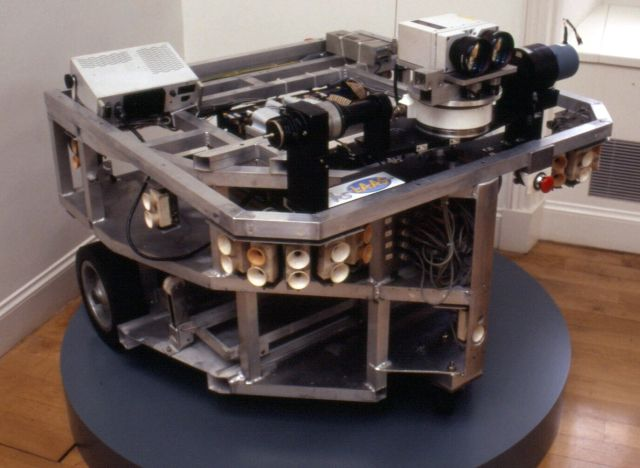
\includegraphics[width=1\columnwidth]{figs/HILARE.png}
\caption{HILARE}
\label{hilare}
\end{figure}

\begin{figure}[H]
\centering
\includegraphics[width=1\columnwidth]{figs/MANIPULADOR.png}
\caption{Manipulador robótico atual}
\label{manipulador}
\end{figure}

\subsection{Arquiteturas deliberativas}
As arquiteturas deliberativas são sistemas hierárquicos com a lógica
\textit{SPA}. São utilizados em sistemas robóticos até hoje, quando a aplicação
favorece seu uso e devido ao grande poder computacional atual. Destacam-se os modelos de Albus,
NASREM, \textit{Nested Hierarchical Controllers} e o \emph{Intelligent Mobile
Robot System} de Saridis.

\subsubsection{Modelo de Albus}

Albus foi o pioneiro e mais influente autor de teorias em arquiteturas
deliberativas, que pode ser vista em \cite{albus1991outline}. Sua
grande contribuição foi a formalização e definição de diversos termos
amplamente utilizados em automação e controle. Dentre outros, destaca-se o
teorema de que há quatro sistemas que compõem a inteligência: processamento de
sensores, modelo do mundo, geração de comportamentos e julgamento de valor. As
entradas desses elementos são os sensores e suas saídas são os atuadores:

\begin{itemize}
  \item Atuadores: as saídas de um sistema inteligente pe produzida por
  atuadores, como mover, posicionar braços, pernas, mãos, olhos e etc. Os
  atuadores naturais são os músculos e as glândulas, já os atuadores de máquinas
  são motores, pistões e válvulas.
  \item Sensores: são as entradas de um sistema inteligente, como sensores de
  força, torque, posição, velocidade, vibração, acústico, gases, temperatura e
  muitos outros. Monitoram o mundo e o estado interno do sistema, e provê dados
  ao sistema de processamento sensorial.
  \item Processamento sensorial: sistema que compara novas observações com a
  expectativa interna do modelo do mundo. Integra e armazena as diferenças e
  semelhanças encontradas, a fim de reconhecer padrões, objetos e relações no
  mundo.
  \item Modelo do mundo: é a melhor estimativa que o sistema inteligente possui
  do mundo, e atualizado pelo processamento sensorial. É um banco de dados com
  todo o conhecimento do mundo e contém uma capacidade de simulação que gera expectativas e predições. O modelo do mundo
  pode prover informações do passado, presente e prevê estados futuros.
  Os dados são importantes para: o gerador de comportamentos escolher o plano
  adequado para execução das ações; o processamento sensorial fazer correlações,
  comparação de modelos, e reconhecimento de objetos, estados e eventos; e o
  sistema de julgamento de valor computar valores de custo, benefício, risco,
  incerteza, importância e outros.
  \item Julgamento de valor: este é o sistema que determina o que é bom ou ruim,
  importante ou trivial, certo ou improvável. Computa custos, riscos e
  benefícios de situações observadas e atividades planejadas.
  \item Gerador de comportamentos: elemento que seleciona objetivos e planos,
  executa e monitora ações, e modifica planos existentes quando alguma situação
  do mundo exigir. Tarefas são decompostas em subtarefas, e subtarefas são
  sequências de objetivos. A ordem lógica de funcionamento é: o gerador de
  comportamentos cria planos, o modelo do mundo predita o resultado do plano, e
  o julgamento de valor avalia os resultados. O gerador de comportamento
  seleciona o plano com a avaliação mais alta.
\end{itemize}
As relações entre os elementos do sistema inteligente estão representados na
figura~\ref{albus}.  Esses elementos e suas relações possibilitaram a criação de
diversas arquiteturas.

\begin{figure}[H]
\centering
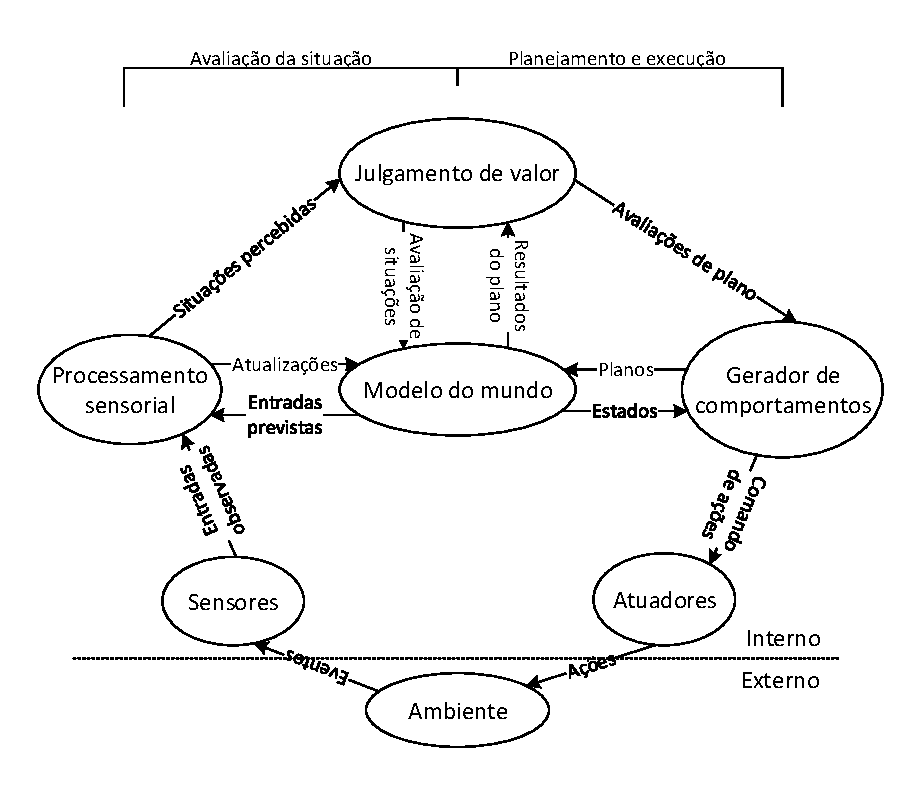
\includegraphics[width=1\columnwidth]{figs/albus.pdf}
\caption{Arquitetura de Albus para sistemas deliberativos.}
\label{albus}
\end{figure}


\subsubsection{NASREM}
O NASREM \cite{albus1989nasa} foi uma arquitetura utilizada pela
NASA e possuía uma arquitetura com seis níveis de
funcionalidade(figura~\ref{nasrem}):

\begin{enumerate}
  \item Servo: provê o controle dos atuadores do robô (posição, velocidade e
  etc).
  \item Primitiva: determina as primitivas de movimento para gerar trajetórias
  suaves.
  \item Movimento elementar: define e planeja trajetórias livre de colisões.
  \item Tarefa: converte ações desejadas de um objeto em sequências de
  movimentos elementares.
  \item Compartimento de serviços: converte ações de grupos de objetos em
  tarefas de um objeto.
  \item Missão: decompõe o plano de missão em alto nível em compartimento de
  serviços.
\end{enumerate}

Vale ressaltar que no modelo NASREM, o operador tem acesso a qualquer nível
hierárquico do robô e pode tomar o controle do robô para si, além de poder
substituir as entradas de sensores, modelo do mundo e outros. Dessa forma, o
nível de autonomia do robô pode ser desenvolvido de forma incremental.

A arquitetura hierárquica proposta em NASREM permite modularidade e propõe uma
metodologia de software.  
 
\begin{figure}[H]
\centering
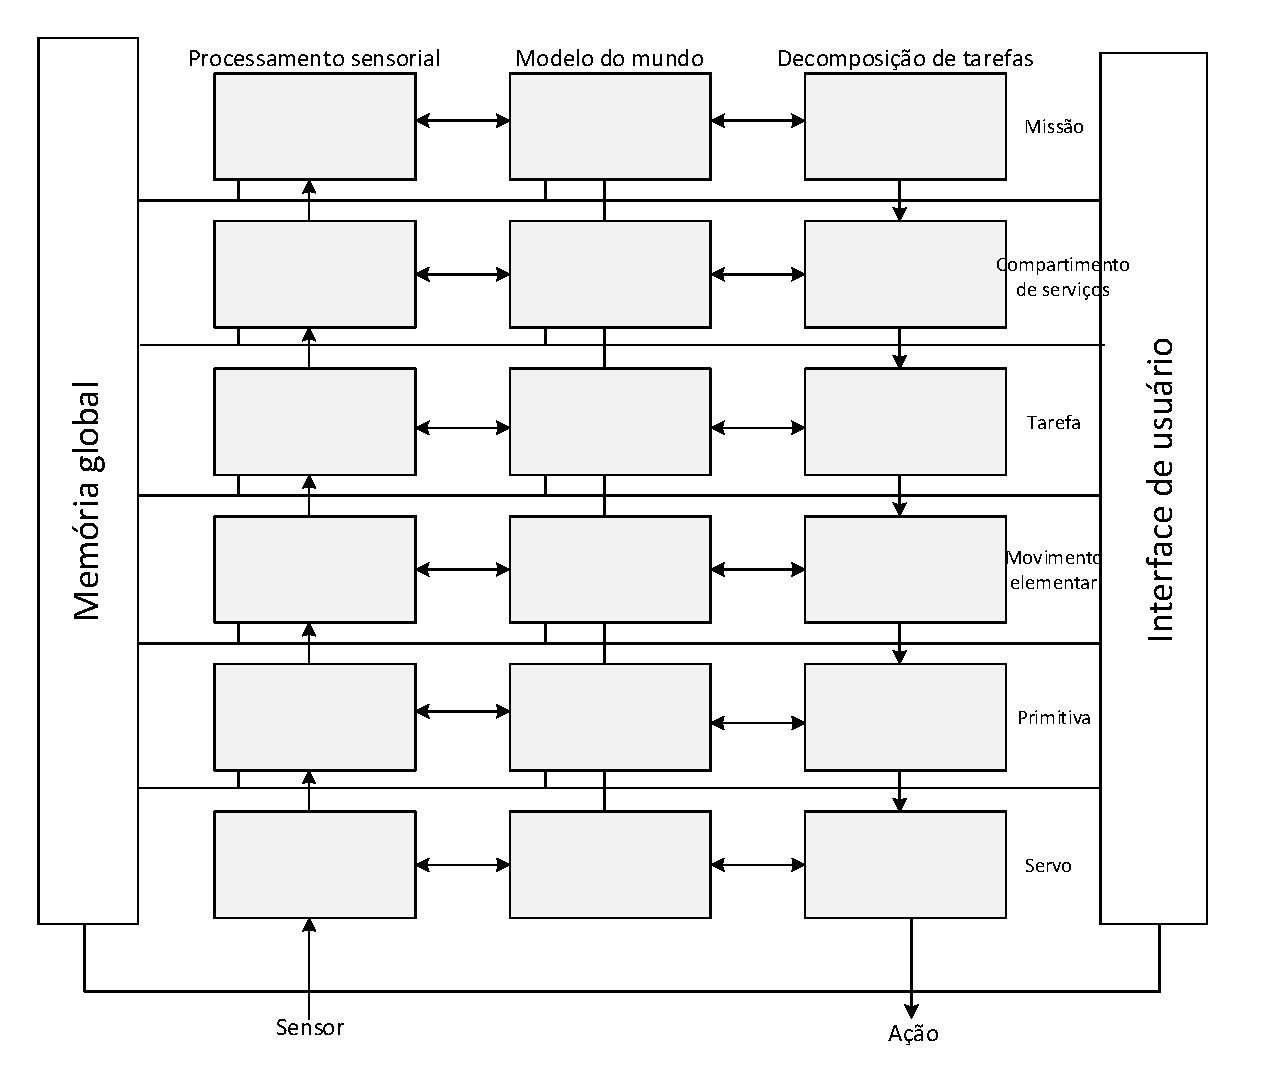
\includegraphics[width=1\columnwidth]{figs/NASREM.pdf}
\caption{Arquitetura NASREM.}
\label{nasrem}
\end{figure}

\subsubsection{\textit{Nested Hierarchical Controllers}}
O \textit{Nested Hierarchical Controllers} (NHC) consiste também em seis
níveis hierárquicos: planejador da missão, navegador, piloto, monitor de
trajetória, controlador, e sistema de controle de baixo nível. Há também
constante atualização do modelo do mundo por um sistema de sensoriamento.

O planejamento é decomposto em planejador da missão, navegador e piloto e seus
módulos são executados sequencialmente, tornando-se mais específico e detalhado.
A lógica é hierárquica: o planejador de missão envia trechos da missão para o
navegador, o qual envia trechos de trajetória para o piloto, que determina ações
ao controlador de baixo nível. A utilização do mapa interno do robô por cada
módulo é diferente, enquanto o planejador usa o mapa global, o piloto recebe
informações locais. Vale observar que, quando o modelo do mundo é atualizado,
muitas vezes não há necessidade de o planejador atualizar toda a missão e
recomeçar o ciclo de planejamento, apenas o piloto pode recalcular a trajetória
local. 
%TODO: FIGURA 

\subsubsection{\textit{Intelligent Mobile Robot System}}
Em 1991, Saridis \cite{wang1991petri} cria o \emph{Intelligent Mobile
Robot System} (IMRS) baseado na teoria de inteligência hierárquica de controle
\cite{saridis1988analytical}. Saridis utiliza redes de Petri como módulos
básicos da arquitetura para traduzir os comandos gerados pelo nível de
organização em algo compreensível para o nível de execução.

O IMRS possui a seguinte arquitetura (figura~\ref{Saridis_1}):
\begin{itemize}
  \item Nível organizacional (organizador de tarefas): gera tarefas de
  movimentação de alto nível.
  \item Nível de coordenação: funciona como uma interface entre o nível
  organizacional e o de execução. O nível é composto por um remetente e alguns
  coordenadores. O remetente recebe o plano da tarefa do organizador, decompõe a
  tarefa em ações de controle e remete aos coordenadores. Os coordenadores
  traduzem os comandos de controle em instruções de operação e transmite ao
  nível de execução.
  \item Nível de execução: executa a instrução proveniente do nível de
  coordenação e reporta seus resultados a ele.
\end{itemize}

\begin{figure}[H]
\centering
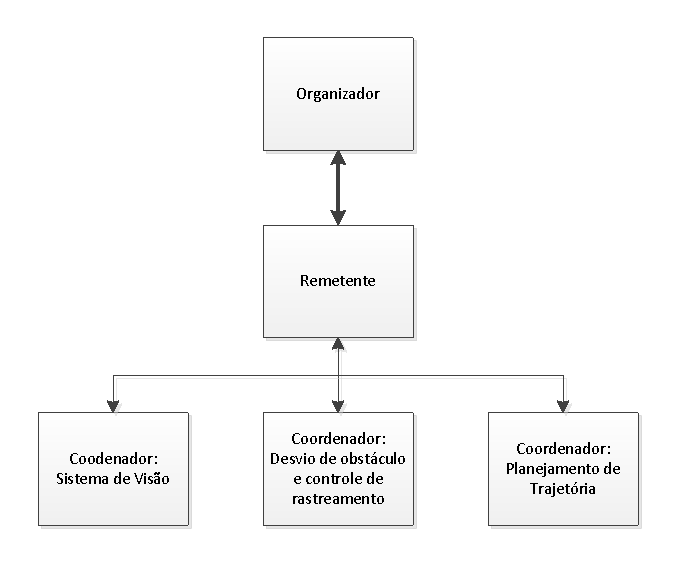
\includegraphics[width=1\columnwidth]{figs/SARIDIS_1.pdf}
\caption{IMRS}
\label{Saridis_1} 
\end{figure}

O nível de coordenação do IMRS é composto por um remetente
(\emph{Dispatcher}) e três coordenadores: sistema de visão (VS), desvio de
obstáculo e controle de rastreamento (OATC), e planejamento de trajetórias (PP).
Com o modelo de redes de Petri não é possível implementar o esquema de linguagem de
decisão para descrever a tradução de tarefas entre remetente e coordenadores.
Portanto, os \emph{Petri Net Transducers} (PNTs) foram introduzidos como
tradutores de linguagem (protocolo): $PNT = (N,\Sigma,
\Delta, \sigma, \mu, F)$. Onde:
\begin{itemize}
	\item A rede de Petri $N=(P,T,I,O)$, $P$ lugares, $T$
transições, função de entrada $I$, função de saída $O$, é o controle da
tradução;
	\item $\mu$ é o estado inicial de $N$;
	\item $\Sigma$ é o alfabeto de entrada, representa tarefas de entradas;
	\item $\Delta$ é o alfabeto de saída, representa tarefas de saída; 
	\item $\sigma$ especifica, para uma dada tarefa de entrada, as transições em
$N$ e as subtarefas de saída que podem ser usadas na tarefa;
	\item $F$ é o estado final. Indica o fim da tradução da tarefa;
\end{itemize}    

Os quatro PNT's são combinados para realizarem a tradução de tarefas no Nível
de Coordenação: remetente, sistema de visão, desvio de obstáculo
e controle de rastreamento, e planejamento de trajetórias. A
figura~\ref{Saridis_2} mostra o modelo de rede de Petri para o Remetente.
%Será brevemente descrito o componente Remetente (\emph{Dispatcher}) do modelo
% de Nível de Coordenação para melhor entendimento do PNT.

%Foram definidas quatro tarefas para o Nível de Coordenação: 1) \emph{wmu}:
%atualização da memória 3-D do ambiente; 2) \emph{mod}: detecção de objetos em
%movimento; 3) \emph{pp}: planejamento de trajetórias; 4) \emph{moac}: desvio de
%obstáculos e controle de rastreamento. A figura~\ref{Saridis_2} mostra o modelo
%de rede de Petri para o Remetente.

\begin{figure}[H]
\centering
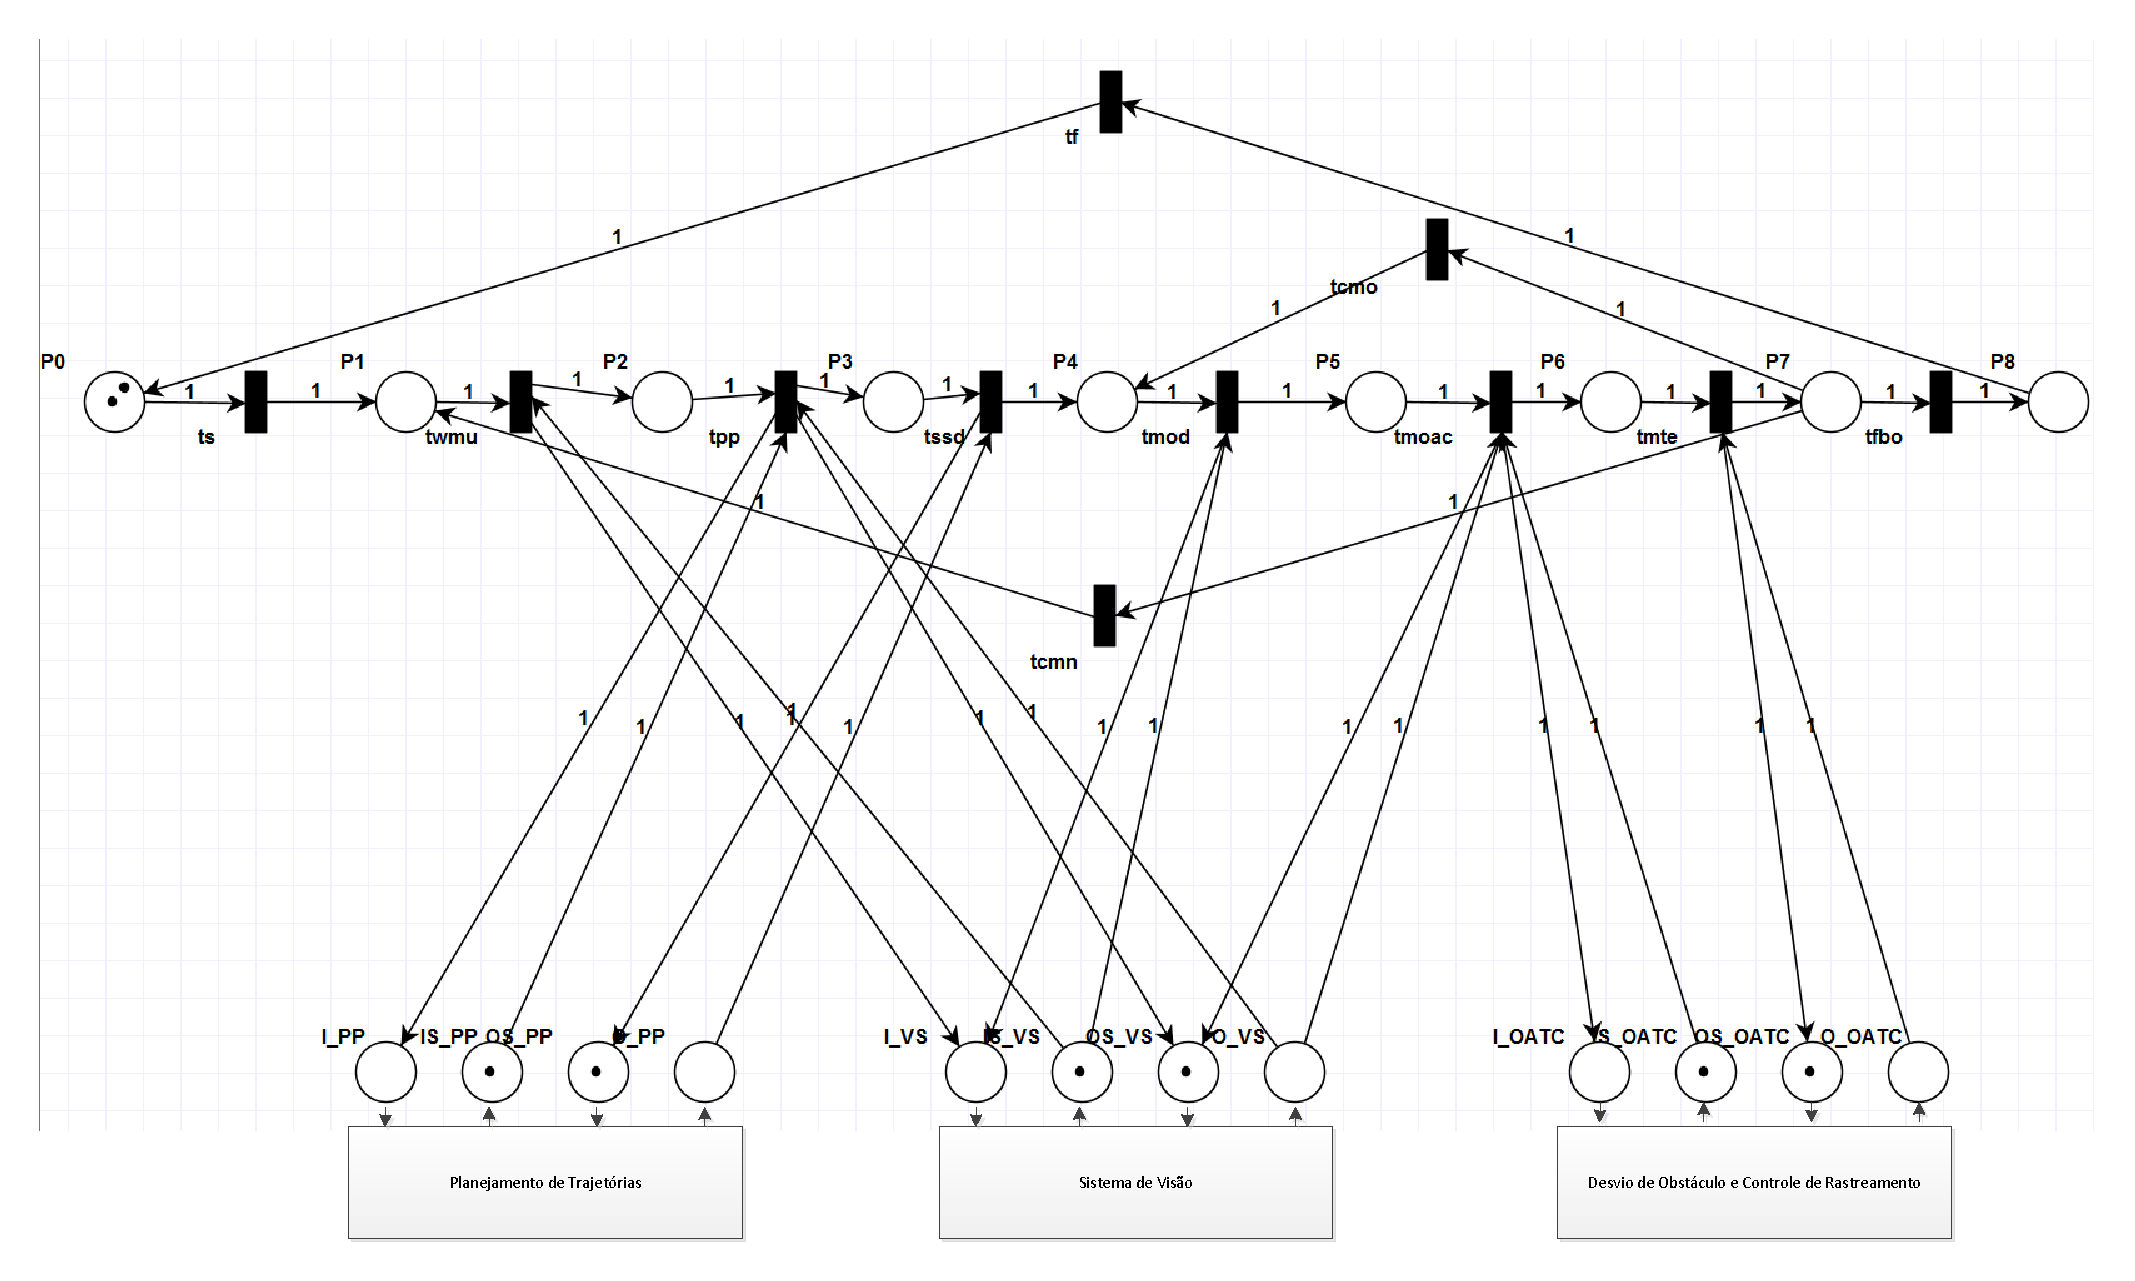
\includegraphics[width=1\columnwidth,angle=90]{figs/SARIDIS_2.pdf}
\caption{Estrutura do nível de coordenação com foco na rede de Petri do
Remetente}
\label{Saridis_2}
\end{figure}

A modelagem do sistema utilizando redes de Petri proporcionaram, como pode ser
visto na figura~\ref{Saridis_2}, algumas funcionalidades essenciais em uma
arquitetura robótica: a capacidade de executar duas tarefas simultaneamente, por
exemplo, movimentação e planejamento de trajetórias; e o \emph{Input Semaphore},
que impede um processo de ser executado até outro ser finalizado.
  
% 
% 
% O estado inicial da rede de Petri é: $$M
% =\{2,0,0,0,0,0,0,0,0,0,1,1,0,0,1,1,0,0,1,1,0\}$$, cujos lugares são: $$M
% =\{P_0,P_1,P_2,P_3,P_4,P_5,P_6,P_7,P_8,I_{PP},IS_{PP},\ldots$$
% $$OS_{PP},O_{PP},I_{VS},IS_{VS},OS_{VS},
% O_{VS},I_{OATC},IS_{OATC},OS_{OATC},O_{OATC}\}$$ 
% As suas transições são:
% \begin{enumerate}
%   \item A transição $t_s$ inicializa o Remetente quando uma tarefa é recebida
%   do Organizador. 
%   $$M=\{1,1,0,0,0,0,0,0,0,0,1,1,0,0,1,1,0,0,1,1,0\}$$  
%   O lugar $P_0$ permanece com um token, logo a transição $t_s$ ainda pode ser
%   disparada. Isso faz com que o Remetente seja capaz de executar duas tarefas
%   simultaneamente: a tarefa de movimentação (ver item 7) e o planejamento de
%   trajetórias (ver item 3).
%   \item A transição $t_{wmu}$ chama o processo de atualização do mapa 3-D. O
%   sistema de visão poderá ser iniciado (token em $I_{VS}$) e a transição
%   $t_{wmu}$ não pode ser disparada novamente até completar mais um ciclo de
%   visão, graças ao \emph{Input Semaphore}, $IS_{VS}$.
%   $$M=\{1,0,1,0,0,0,0,0,0,0,1,1,0,1,0,1,0,0,1,1,0\}$$
%   Ao fim do ciclo do sistema de visão, o seu \emph{Output Point}, $O_{VS}$,
%   adquire um token, habilitando a transição $t_{PP}$ do Remetente. 
%   $$M=\{1,0,1,0,0,0,0,0,0,0,1,1,0,0,1,0,1,0,1,1,0\}$$
%   Vale observar que não é possível modelar essas características com máquinas de
%   estado sem a utilização de recursos extras como inibidores e supressores.
%   \item A transição $t_{pp}$ habilita o planejamento de trajetórias (token em
%   $I_{PP}$), com restrições de espaço, cinemática, dinâmica e critério de
%   otimização. $t_{pp}$ não pode ser disparada novamente até completar um
%   ciclo de planejamento de trajetórias, graças ao \emph{Input Semaphore},
%   $IS_{PP}$.
%   $$M=\{1,0,0,1,0,0,0,0,0,1,0,1,0,0,1,1,0,0,1,1,0\}$$
%   Ao fim do ciclo do planejamento de trajetórias, o seu \emph{Output
%   Point}, $O_{PP}$, adquire um token, habilitando a transição $t_{ssd}$ do
%   Remetente.
%   $$M=\{1,0,0,1,0,0,0,0,0,0,1,0,1,0,1,1,0,0,1,1,0\}$$
%   \item A transição $t_{ssd}$ é disparada para colocar o estado do planejamento
%   de trajetórias no valor inicial:
%   $$M=\{1,0,0,0,1,0,0,0,0,0,1,1,0,0,1,1,0,0,1,1,0\}$$
%   \item A transição $t_{mod}$ é disparada para o desvio de obstáculo em um
%   espaço especificado e provê acurácia e tempo requerido. O
%   sistema de visão poderá ser iniciado novamente (token em $I_{VS}$) e a
%   transição $t_{mod}$ não pode ser disparada novamente até completar mais um
%   ciclo de visão, graças ao \emph{Input Semaphore}, $IS_{VS}$.
%   $$M=\{1,0,0,0,0,1,0,0,0,0,1,1,0,1,0,1,0,0,1,1,0\}$$
%   Ao fim do ciclo do sistema de visão, o seu \emph{Output Point}, $O_{VS}$,
%   adquire um token, habilitando a transição $t_{moac}$ do Remetente. 
%   $$M=\{1,0,0,0,0,1,0,0,0,0,1,1,0,0,1,0,1,0,1,1,0\}$$
%   \item A transição $t_{moac}$ é disparada e habilita o desvio de obstáculo
%   e controle de rastreamento (token em $I_{OATC}$). O estado do sistema de visão volta para
%   o valor inicial e $t_{moac}$ não pode ser disparada novamente até completar um
%   ciclo de desvio de obstáculo, graças ao \emph{Input Semaphore}, $IS_{OATC}$.
%   $$M=\{1,0,0,0,0,0,1,0,0,0,1,1,0,0,1,1,0,1,0,1,0\}$$
%   Ao fim do ciclo do desvio de obstáculo, o seu \emph{Output
%   Point}, $O_{OATC}$, adquire um token, habilitando a transição $t_{mte}$ do
%   Remetente.
%   $$M=\{1,0,0,0,0,0,1,0,0,0,1,1,0,0,1,1,0,0,1,0,1\}$$
%   \item A transição $t_{mte}$ realiza a tarefa de movimentação do robô. O
%   sistema de desvio de obstáculos e controle de rastreamento volta para o estado
%   inicial.
%   $$M=\{1,0,0,0,0,0,0,1,0,0,1,1,0,0,1,1,0,0,1,1,0\}$$
%   Caso haja falha, as transições $t_{cmo}$ ou $t_{cmn}$ podem ser disparadas.
%   \item A transição $t_{fbo}$ dispara para o envio de \emph{feedbacks} ao
%   Organizador.
%   $$M=\{1,0,0,0,0,0,0,0,1,0,1,1,0,0,1,1,0,0,1,1,0\}$$
%   \item A transição $t_{cmn}$ é disparada em caso de falha na movimentação do
%   robô. O robô continuará o seu movimento por um novo caminho. Volta ao item 2.
%   $$M=\{1,1,0,0,0,0,0,0,0,0,1,1,0,0,1,1,0,0,1,1,0\}$$ 
%   \item A transição $t_{cmo}$ é disparada em caso de falha na movimentação do
%   robô. O robô continuará o seu movimento pelo mesmo caminho. Volta ao item 5.
%   $$M=\{1,0,0,0,1,0,0,0,0,0,1,1,0,0,1,1,0,0,1,1,0\}$$
%   \item A transição $t_f$ dispara para reportar o resultado da movimentação do
%   robô ao Organizador. Volta ao item 1.
%   $$M=\{2,0,0,0,0,0,0,0,0,0,1,1,0,0,1,1,0,0,1,1,0\}$$ 
% \end{enumerate} 

%A rede de Petri evidencia o motivo do uso dos PNT, com os parâmetros aumentados
%$PNT = (N,\Sigma, \Delta, \sigma, \mu, F)$. %Até agora, apenas as variáveis
%diretamente ligadas à rede: $N$ e $\mu$ foram analisadas, mas quando se busca a
%Quando se busca a integração das redes dos coordenadores fica nítida a
% necessidade de parâmetros para especificação das tarefas.

%O alfabeto de entrada do Remetente é dado pelo Organizador, dado como
%$\Sigma_0$. O alfabeto de saída ($\Delta_0$) são os alfabetos de entrada para
%cada coordenador (PP, VS e OATC): $\Sigma_p = \{path\}$,
%$\Sigma_m=\{\textrm{freemove}, \textrm{move}\}$ e
%$\Sigma_v=\{\textrm{sendinfo.detection}, \textrm{terrain}\}$.

%O parâmetro que especifica as transições para uma determinada tarefa e as
%subtarefas é o $\sigma$. Para a transição $t_{mod}$, por exemplo,
%$\sigma(t_{mod},mod)=\{\textrm{detection.sendinfo}(ard_i,ptc_i),
%\textrm{sendinfo}(ard_i,ptc_i)\}$, onde $ard$ é a acurácia requerida sobre
%objetos detectados em VS e $ptc$ é o tempo para a realização do processo. A
% rede de Petri no coordenador VS pode, portanto, assumir transições paralelas (dois
%caminhos) e o que define qual caminho deve ser seguido é o parêmetro do
%Remetente (neste caso será a transição $t_{smd}$ de VS).

Saridis salienta os benefícios das PNT:
\begin{itemize}
  \item Redes de Petri podem ser usadas como módulos básicos para sistemas de
  controle de missão de robôs móveis.
  \item A comunicação e conexão de módulos são eficientes entre redes de Petri.
  \item Controle e mecanismo de comunicação para coordenação de tarefas de um
  robô móvel podem ser realizados com redes de Petri.
\end{itemize} 

A arquitetura de Saridis é uma contribuição importante por criar um nível
organizacional, separando o nível do desenvolvedor de baixo nível e um
nível de alto nível para um operador (usuário). Além disso, as redes de Petri
assumem um importante papel como módulo básico de controle para seu sistema
IMRS. As redes de Petri foram originalmente introduzidas para descrever as
comunicações de máquinas de estado finito (FSM), possibilitando flexibilidade
e robustez, e é provado que redes de Petri são excelente ferramenta para
modelagem de sistemas, sobretudo quando envolvem tarefas conflitantes ou
simultâneas, Murata \cite{murata1989petri}.


\subsection{Análise crítica}
A abordagem deliberativa simula, de certa forma, o processo de planejamento e
tomada de decisão do ser humano. Há um núcleo (cérebro) que
processa todos os dados sensorias e armazena o mundo, isto é, o ambiente em que
está inserido, de maneira simbólica, geométrica ou outras.
Além disso, ele planeja todas as ações para uma determinada tarefa, consultando sua ideia de mundo intensivamente. Há,
também, sensores que enviam suas novas informações periodicamente para o núcleo,
(órgãos receptivos: visão, olfato, e etc), atualizando o mundo. E há
atuadores (músculos) necessários para a realização das tarefas~\ref{brain}.

É fácil observar que a arquitetura deliberativa é dependente do
modelo de mundo armazenado e suas atualizações periódicas. Portanto, a
utilização da abordagem deliberativa em ambientes extremamente dinâmicos pode ser muito
custosa devido às atualizações e ao replanejamento. Além disso, é fácil observar
que a arquitetura SPA dificulta a criação de sistemas em tempo real eficientes.

\begin{figure}[H]
\centering
\includegraphics[width=1\columnwidth]{figs/BRAIN.png}
\caption{Comparativo da arquitetura deliberativa com o ser humano.}
\label{brain}
\end{figure}

\section{Paradigma reativo}

Sistemas de arquitetura reativa também são chamados de sistemas baseados em
comportamentos. Os robôs são programados para agir através de ativação de uma
coleção de comportamentos primitivos de baixo nível. De acordo com
\cite{arkin1995reactive}, as principais características de sistemas puramente
reativos são:

\begin{itemize}
  \item Comportamentos são como elementos construtivos: são um par sensor-motor,
  onde o sensor provê informação necessária para o motor executar uma ação
  reativa, como desvio de obstáculo, atrair-se a objetivos, escapar de
  predadores e etc.
  \item Não há criação ou manutenção precisa do modelo do mundo. Os sistemas
  reagem ao estímulo do mundo, extremamente útil para mundos dinâmicos e
  hostis.
  \item Comportamentos de animais são normalmente utilizados para modelar esses
  sistemas.
\end{itemize}

Dessa forma, controle reativo é uma técnica que une percepção e ação,
tipicamente no contexto de comportamentos motores, para produzir respostas
robóticas em tempo real em mundos dinâmicos e não estruturados.

Em 1986, um dos primeiros estudos em sistemas reativos foi desenvolvido por
Rodney Brooks \cite{brooks1986robust}. Este estudo é a base para diversos
trabalhos atuais que envolvem robôs reativos móveis. Os desafios de
robôs autônomos apontados por Brooks e que ainda ilustram os problemas da
atualidade são: \emph{múltiplos objetivos}, \emph{múltiplos sensores},
\emph{robustez} e \emph{extensibilidade}. De acordo com Brooks, esses desafios
não são suportados pela arquitetura tradicional (paradigma hierárquico) de um
sistema de controle.

Os múltiplos objetivos de robôs móveis podem:
\begin{itemize}
  \item Ser conflitantes: por exemplo, um robô pode estar tentando alcançar um
  determinado ponto no espaço, porém evitando obstáculos locais.
  \item Ter relações de prioridade: por exemplo, um robô que inspeciona trilhos
  de trêm deve sair dos trilhos ao ouvir o sinal de um trêm chegando, mesmo se estiver
  finalizando a operação.
  \item Ser denpendentes: objetivos de \emph{alto nível} englobam diversos
  objetivos de \emph{baixo nível}. No caso do exemplo acima, o robô que sai do
  trilho para evitar o trêm deve se manter equilibrado para não cair. Artigos
  recentes, como em \cite{fryxell1996navigation} separam esses objetivos em
  \emph{tarefas} (objetivos de \emph{alto nível}) e \emph{primitivas do veículo}.
\end{itemize}

Robôs são normalmente providos de múltiplos sensores e suas diversas
informações podem ser redundantes, conflitantes ou complementares,
podendo ser utilizadas para uma mesma tarefa do robô.
Por exemplo, encoders para odometria e câmeras fixas ao robô
podem ser utilizados para localização, de forma que se complementem.
Os sensores podem apresentar erros ou resultados conflitantes, portanto a fusão
da informação de múltiplos sensores, a determinação de seus graus de
confiabilidade e em quais tarefas devem ser considerados são decisões que o
robô deve saber fazer.

Um robô deve ser robusto, isto é, em caso de falha de um sensor, o robô
deve se adaptar e utilizar os outros sensores que ainda funcionam para realizar as
tarefas. Ou em caso de alterações no ambiente, o robô deve ser
capaz de cumprir determinadas funções essenciais.

A extensibilidade constitui em acrescentar mais sensores e,
portanto, aumentar a capacidade do robô, sendo possível a execução de novas
tarefas. Porém, existe um limite imposto pela limitação
de processamento do robô, já que um novo hardware (sensor) é adicionado, mas o
processamento (computador) não é substituído e sua capacidade não é aumentada.

Brooks propõe um dos primeiros sistemas baseados em comportamentos, uma
arquitetura que tem como objetivo descentralizar a tomada de decisão de um
modelo central, como pode ser visto na figura~\ref{BROOKS_1}. O autor comenta
que essa decomposição conduz a uma arquitetura radicalmente diferente para
sistema de controle de robôs móveis em estratégias de implementação a nível de
hardware e com grandes vantagens em robustez, desenvolvimento e teste.

\begin{figure}[H]
\centering
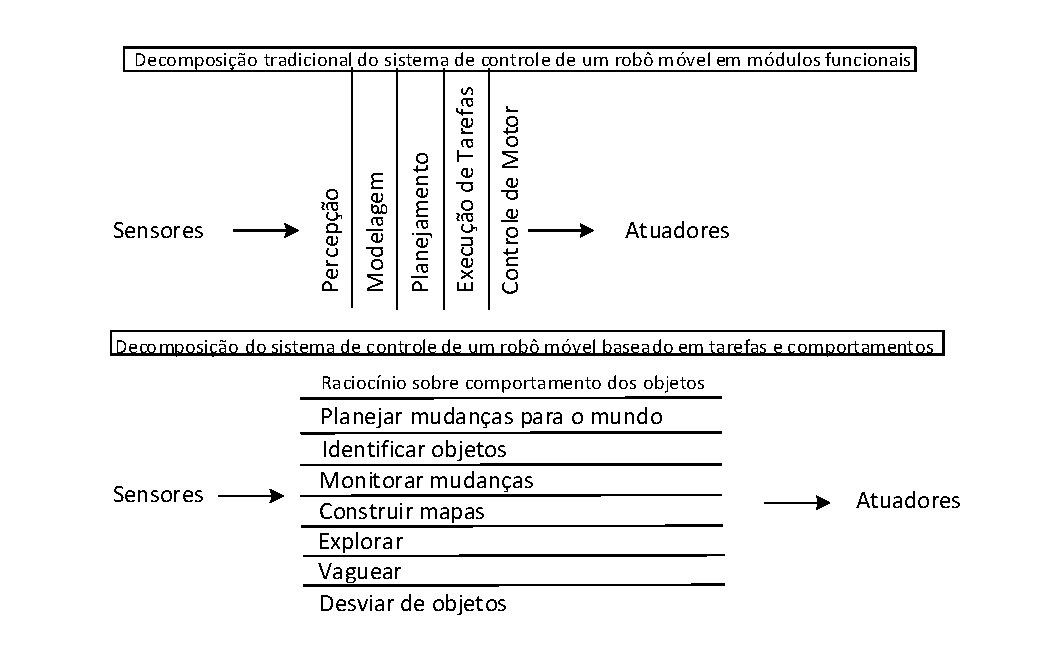
\includegraphics[width=1\columnwidth]{figs/BROOKS_1.pdf}
\caption{Arquitetura para sistema de controle de robôs móveis por Brooks}
\label{BROOKS_1}
\end{figure}

\subsection{Robôs reativos}
Antes mesmo de Brooks, ou seja, da formalização de toda a teoria em sistemas
reativos, simples robôs eram criados na lógica de controle reativo e de
comportamentos. Em 1953, por exemplo, Grey Walter \cite{holland1997grey}
desenvolveu uma ``tartaruga'' elétrica capaz de se movimentar pelo ambiente,
evitando luz intensa (``ameaças'') e atraída por certos objetivos. Vale
observar a característica do robô de perceber baixo nível de bateria e procurar
uma estação de recarga, comportamento que se sobrepõe aos outros. Os
comportamentos são simples e não há representação abstrata do mundo:
dirigir-se para luz fraca; fugir de luz forte; e evitar obstáculos.

Em 1984, veículos simples e puramente reativos com os pares clássicos
sensor-motor foram desenvolvidos pelo psicologista Braitenberg
\cite{braitenberg1986vehicles}, a fim de simular sentimentos, como covardia,
agressividade e outros. 

Em 2002 até os dias atuais, o robô iRobot Roomba ganha destaque comercial e
executa uma simples tarefa doméstica: limpar o chão. Em sua arquitetura, o robô
Roomba possui apenas algumas funções reativas, como esquivar-se e locomover-se,
e, em suas versões antigas, foi constatado que não possui o modelo do mundo,
mapa, dentro de si \cite{tribelhorn2007evaluating}.

\subsection{Arquiteturas reativas}


\subsubsection{Arquitetura de subsunção}
Na figura~\ref{BROOKS_1}, o autor define \emph{Níveis de competência}, que são
classes de comportamentos desejados para o robô sobre todos os ambientes que ele
pode encontrar. As classes definidas por Brooks são:
\begin{enumerate}
\setcounter{enumi}{-1}
  \item Evitar contato com objetos (estacionários ou móveis);
  \item Vaguear sem rumo e sem bater em objetos;
  \item Explorar o ambiente utilizando sensores e definir lugares alcançáveis.
  Seguir rumo em sua direção;
  \item Construir um mapa do ambiente e planejar trajetórias de um lugar para
  outro;
  \item Observar mudanças no ambiente;
  \item Raciocinar sobre o ambiente em termos de objetos identificáveis e
  realizar tarefas relacionadas a certos objetos;
  \item Formular e executar planos que envolvam mudar o estado do ambiente como
  desejado;
  \item Raciocinar sobre o comportamento de objetos no ambiente e modificar
  planos quando necessário;
\end{enumerate}

Vale observar que cada nível de competência inclui, como subconjunto, os
níveis de competência anteriores.

Após a decomposição na nova arquitetura, Brooks define as \emph{Camadas de
Controle}, correspondentes a cada nível de competência. A ideia dessa abordagem
é adicionar camadas de controle a níveis de competências superiores sem precisar
alterar a camada do nível inferior. Inicia-se, portanto, com a camada de
controle para o nível zero de competência, esta será testada e não mais
alterada. Após, é criada a camanda de nível 1, capaz de examinar os dados
da camada de nível 0 e injetar dados nas interfaces internas deste nível,
suprimindo seu trânsito de dados, figura~\ref{BROOKS_2}.

\begin{figure}[H]
\centering
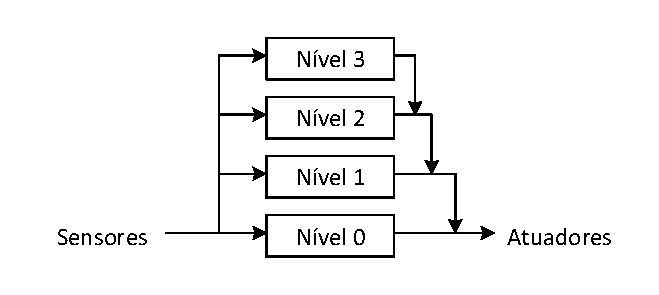
\includegraphics[width=1\columnwidth]{figs/BROOKS_2.pdf}
\caption{Camadas de controle de Brooks}
\label{BROOKS_2}
\end{figure}

Os problemas apresentados por Brooks são solucionados pela nova arquitetura:
\begin{itemize}
  \item Múltiplos objetivos: camadas individuais podem trabalhar em objetivos
  individuais ao mesmo tempo. Os níveis das camadas de controle e o mecanismo de
  supressão do trânsito de dados resolvem os problemas de conflito, dependência
  e prioridade;
  \item Múltiplos sensores: as camadas utilizam os dados dos sensores
  independentemente, de forma que não há necessidade de se preocupar com a
  fusão;
  \item Robustez: além do uso inteligente de sensores, camadas de controle de
  nível inferior continuam a funcionar quando novas camadas de nível superior
  são adicionadas;
  \item Extensibilidade: cada camada de controle pode possuir o seu próprio
  processador; 
\end{itemize}

A estrutura das camadas de controle foram construídas por um conjunto de
pequenos processadores que enviam mensagens uns para os outros. Cada processador
é uma máquina de estado finito. A nova arquitetura e essa nova estrutura de
camadas com eventos discretos foram a base de diversos sistemas de controle de
missão da atualidade. A fim de melhorar o entendimento desse sistema criado
por Brooks, serão apresentados dois níveis de seu controle em uma aplicação de robô
móvel.

A camada de controle nível zero deve garantir que o robô não entre em contato
com outros objetos, estacionários ou móveis. Portanto, o robô deve desviar de
objetos que se aproximam ou parar se houver um objeto fixo em sua trajetória.
Na figura~\ref{BROOKS_3}, podemos observar o nível 0 de controle do sistema.

\begin{figure}[H]
\centering
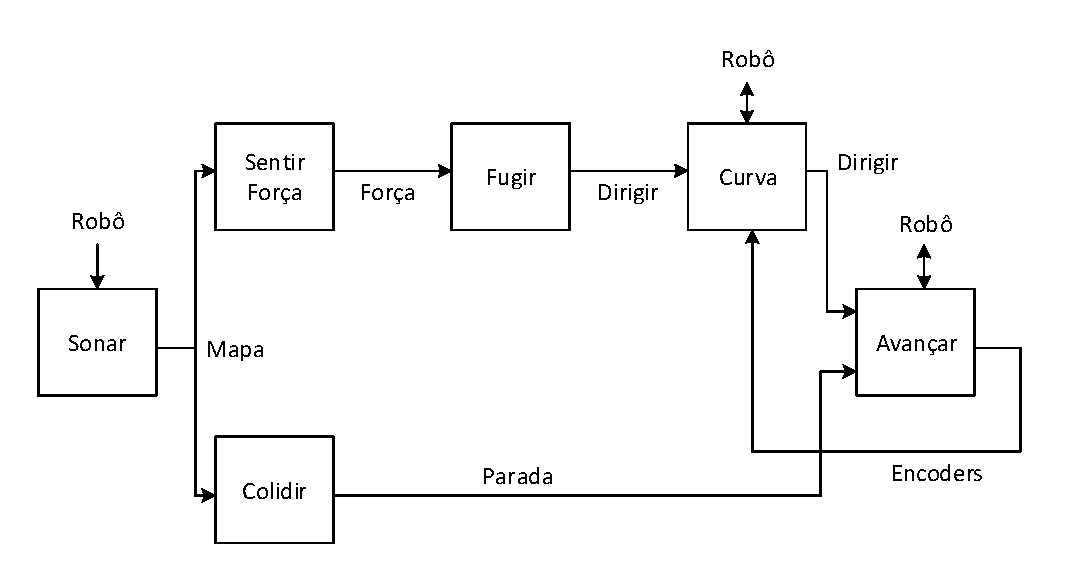
\includegraphics[width=1\columnwidth]{figs/BROOKS_3.pdf}
\caption{Nível 0 de controle do sistema}
\label{BROOKS_3}
\end{figure}

Segue pequena descrição de cada módulo:
\begin{itemize}
  \item Módulo \emph{Curva}: comunica-se diretamente com o robô (atuadores).
  Recebe uma mensagem \emph{Dirigir} especificando um ângulo de giro seguido por
  uma mensagem do módulo \emph{Avanço} com uma determinada magnitude. Isso faz
  com que o robô realize uma curva e vá para o estado de \emph{Avanço}.
  \item Módulo \emph{Avanço}: comando faz robô se movimentar (atuadores), mas
  pára o robô se receber mensagem do módulo \emph{Colisão}. O robô fica inativo
  e mensagens do encoder é enviado ao módulo \emph{Curva}, funcionando como um
  \emph{reset}, e podendo receber novos comandos.
  \item Módulo \emph{Sonar}: recebe um vetor de informações de sensores do robô,
  filtra os dados e produz um mapeamento de obstáculos para o robô em
  coordenadas polares.
  \item Módulo \emph{Colisão}: monitora o mapa gerado pelo módulo \emph{Sonar}
  e, se detectar um obstáculo, envia um sinal de parada. Observe que este módulo
  funciona independentemente se o robô está em movimento ou parado.
  \item Módulo \emph{Sentir Força}: cada obstáculo detectado é somado
  como uma força repulsiva, gerando uma força resultante.
  \item Módulo \emph{Fugir}: monitora a força produzida pelos obstáculos e envia
  comandos para o módulo \emph{Curva} se a força for significante.
\end{itemize}
 
 A camada de controle nível 1, combinada a camada de controle nível 0, permite
 que o robô vagueie sem colisões. A figura~\ref{BROOKS_3} mostra o sistema de
 controle aumentado pelo nível da camada 1.

\begin{figure}[H]
\centering
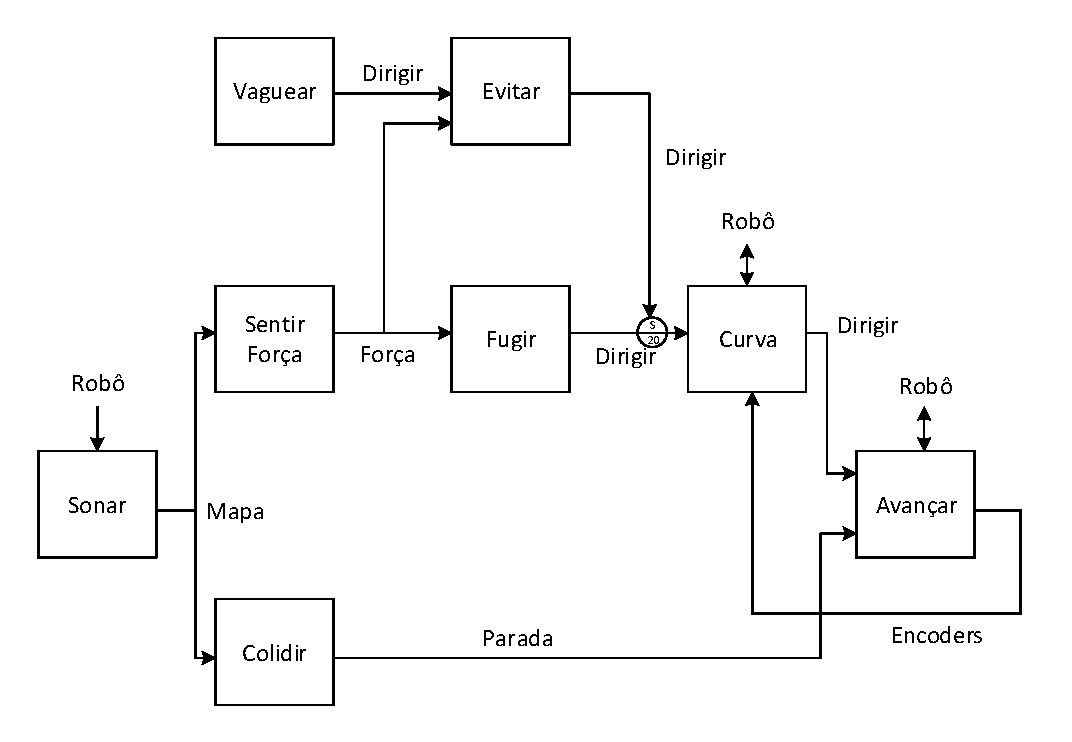
\includegraphics[width=1\columnwidth]{figs/BROOKS_4.pdf}
\caption{Nível 0 e 1 de controle do sistema}
\label{BROOKS_4}
\end{figure}

Segue pequena descrição de cada módulo do nível 1:
\begin{itemize}
  \item Módulo \emph{Vaguear}: gera nova direção para o robô a cada 20 segundos.
  \item Módulo \emph{Evitar}: recebe resultado da força computada pelo nível 0
  de controle e combina com a direção desejada pelo módulo \emph{Vaguear},
  produzindo uma nova direção desejada sem obstáculos. Esse resultado presume as
  computações do módulo \emph{Fugir}. Vale observar que o módulo \emph{Evitar}
  suprime a saída do módulo \emph{Fugir} (mecanismo de supressão). 
\end{itemize}

A nova arquitetura de Brooks é robusta, permite interações dinâmicas, é flexível
para integrar novas funcionalidades e fácil para implementar e debugar. Brooks
ainda associa sistemas de eventos discretos no controle de robôs autônomos,
utilizando como módulos básicos máquinas de estados finitos (FSM - \emph{Finite
State Machine}). Como a conexão de diversas FSM's não é uma FSM, a solução
encontrada por Brooks foi acrescentar inibidores e supressores em suas
FSM, chamando-as AFSM (\emph{Augmented Finite State Machine} ou máquina de
estado aumentada). O módulo principal desta arquitetura pode ser visto na FIGURA
%TODO Colocar figura de brooks 



Antes de Brooks, em 1983, Elfes, A. \cite{elfes1983distributed},já havia
idealizado uma arquitetura em módulos e controle distribuído a fim de atingir efetividade em processamento
paralelo, flexibilidade de interação com os diversos sensores, distribuir
capacidades de decisão e flexibilidade de expansão e modificação do sistema.
Porém o sistema de comunicação entre módulos era centralizado
(\emph{Blackboard}) e só realizavam uma determinada tarefa sob o comando de um
Plano de Controle (\emph{Control Plan}). O usuário ainda deveria explicitamente
codificiar paralelismo, os casos das exceções e condições inesperadas.

Apesar dos pontos positivos, a arquitetura de controle de um sistema
baseado em comportamento apresenta problemas com escala e contextualização
(\emph{situatedness}). 

O problema com escala é resultado das interconexões, que
podem crescer de maneira fatorial em relação ao número de comportamentos. 
A contextualização é um problema de sistemas de subsunção, onde subsistemas são
incluídos em um sistema mais amplo. Como cada comportamento é uma FSM, operando
concorrentemente com as outras, o comportamento corrente é o único estado no
qual o veículo como um todo funcionará. São sistemas também chamados de
\emph{non-taskable systems} - uma tarefa não pode ser designada ao
veículo sem reprogramação de todo o sistema.  

Apenas em 1996, Bellingham e Consi \cite{bellingham1994second}
propuseram um controle por camadas (\emph{Layered Control}) a fim de resolver o
problema de escala. A diferença entre o controle baseado em comportamento e o de
Bellingham é a restrição de interatividade entre camadas.

As camadas (que são referenciadas como comportamentos) são associadas com um número de
prioridade, de forma que saídas conflitantes são resolvidas com esse número. Há
um módulo de processamento de sensores que disponibiliza os dados aos
comportamentos, como o \emph{Blackboard}, o que viola a premissa de
paralelismo, mas resolve o problema de interconexões, já que antes as camadas
superiores deveriam se conectar às inferiores para obter os dados dos sensores.

A solução para o problema de contextualidade só foi resolvido em 2000 por Bennet
\cite{bennett2000behavior}. No \emph{State Configured Layered Control} (SCLC),
múltiplos conjuntos de comportamentos simples são escolhidos de uma biblioteca
de comportamentos e são executados em cada fase da missão. A vantagem é o
número reduzido de comportamentos sendo executados ao mesmo tempo. Veremos mais
a frente que esta estratégia é muito realizada em controle híbrido.

% Em 1989, Chatila \cite{norelis1989control} descreve uma nova arquitetura e
% sistema de controle utilizando, assim como Brooks, módulos hierárquicos. A
% arquitetura do robô pode ser decomposta da seguinte forma:
% \begin{itemize}
%   \item \textbf{Módulos de sensores}: processam as saídas dos sensores. Os dados
%   adquiridos por um sensor são processados pelo módulo de sensor e ficam
%   disponíveis para os módulos de nível mais alto para seus próprios
%   processamentos e interpretaçõs.
%   \item \textbf{Unidades funcionais}: realizam uma determinada função no robô.
%   Por exemplo, localização do robô combinando sensores de visão, odometria, laser e
%   etc.
%   \item \textbf{Processos}: realiza a dinâmica de malha fechada entre percepção
%   e ação, usando unidades de função. O processo é representado por uma máquina de estado
%   finito, onde suas entradas são os dados dos módulos dos sensores e suas saídas
%   são comandos aos atuadores.
% \end{itemize}
% 
% O sistema de controle de Chatila é composto por quatro componentes: Supervisor
% (não implementado), Módulo Executivo, Gerente de Vigilância e Módulo de
% Diagnóstico (não implementado). Os controles funcionam como um \emph{if - then},
% com diversas condições e ações predeterminadas. O módulo de vigilância é
% responsável por:
% 
% \begin{itemize}
%   \item Indicar estados dos sensores e tomar ações de reflexo;
%   \item Indicar estado operacional do robô, como nível da bateria;
%   \item Relatar plano e estado da missão que está sendo executada pelo robô;
% \end{itemize}
% 
% O módulo executivo fucniona como um sistema operacional. Recebe comandos
% (missões) predefinidas pela interface e se comunica com o módulo de vigilância.
% 
% Quando comparamos com Brooks, Chatila apresenta uma estrutura bem
% rudimentar e lógicas simples de arquitetura e controle. Apesar de utilizar a
% ideia de recursos compartilhados nos módulos de sensores, os automatos dos
% módulos de processo são bem simplificados e dependentes de um bloco central
% para resolver objetivos conflitantes.

\subsection{Análise crítica}
Se a abordagem deliberativa simulava o processo de planejamento e tomada de
decisão do ser humano, os sistemas de arquitetura reativa simulam outra
importante função da medula espinhal, pertencente ao nosso sistema nervoso
central: o circuito reflexivo, ou arco reflexo. O reflexo é uma resposta
involuntária rápida, consciente ou não, originado de um estímulo externo e
realizada antes mesmo de o cérebro tomar conhecimento do estímulo periférico.



Dessa forma, não há planejamento,  Há um núcleo (cérebro) que processa todos os
dados sensorias e armazena o mundo, isto é, o ambiente em que está inserido, de maneira simbólica, geométrica ou outras.
Além disso, ele planeja todas as ações para uma determinada tarefa, consultando sua ideia de mundo intensivamente. Há,
também, sensores que enviam suas novas informações periodicamente para o núcleo,
(órgãos receptivos: visão, olfato, e etc), atualizando o mundo. E há
atuadores (músculos) necessários para a realização das tarefas~\ref{brain}.

É fácil observar que a arquitetura deliberativa é dependente do
modelo de mundo armazenado e suas atualizações periódicas. Portanto, a
utilização da abordagem deliberativa em ambientes extremamente dinâmicos pode ser muito
custosa devido às atualizações e ao replanejamento. Além disso, é fácil observar
que a arquitetura SPA dificulta a criação de sistemas em tempo real eficientes.

\begin{figure}[H]
\centering
\includegraphics[width=1\columnwidth]{figs/BRAIN.png}
\caption{Comparativo da arquitetura deliberativa com o ser humano.}
\label{brain}
\end{figure}


\section{Arquitetura híbrida deliberativa/reativa}



A partir de 1995, os autores começam a introduzir formalismo e terminologias
para os sistemas que visam o controle de missão de robôs. 

Em 1995, Espiau, B. [9] (INRIA, França), define sistemas híbridos como sistemas
que nem são puramente tempo contínuo, nem máquina de estado finito, mas que
combinam eventos discretos e componentes contínuos. Esses sistemas foram
estudados por duas comunidades distintas: ciência da computação e controle e
automação. Engenheiros de controle e automação estudam sistemas dinâmicos
(modelos) com ênfase nas teorias de estabilidade, convergência, robustez e
introduzem sistemas de eventos discretos para mudanças no controle ou no modelo.
A ciência da computação faz o caminho inverso: um estado em uma máquina de
estados representa um local de controle, onde variáveis mudam continuamente com
o tempo, de acordo com leis de evolução. As ideias de controle híbrido são
desenvolvidas desde Brooks e aparece, mesmo que de forma rudimentar, nos
trabalhos apresentados anteriormente neste documento. 

A contribuição de Espiau foi o desenvolvimento do ORCCAD, um sistema híbrido
para especificação, validação, simulação e implementação de aplicações
robóticas. O sistema possui os seguintes princípios:

\begin{itemize}
  \item Tarefas físicas podem ser tratadas como problemas de controle, os quais
  são resolvidos em tempo real utilizando técnicas de realimentação em controle.
  A abordagem \emph{Task-Function} foi desenvolvida em [10].
  \item A caracterização de uma ação física não é suficiente para definir
  completamente a ação de um robô: tempo inicial e final devem ser considerados,
  assim como as ações que o robô deve tomar em caso de eventos observados
  durante a execução de alguma tarefa.
  \item Como a performance de um sistema depende da eficiência de mecanismos em
  tempo real no nível de operação, deve-se ter atenção particular em sua
  especificação e verificação.
\end{itemize}

No sistema híbrido, o interesse do usuário final é em sua aplicação, portanto
o sistema deve prover formalismo de alto nível para o usuário focar em
especificação e verificação de tarefas. Por outro lado, o engenheiro
de controle necessitará de um ambiente de programação, desenvolvimento e
simulação para expressar suas leis de controle, as quais são encapsuladas para
o usuário final. No ORCCAD, duas entidades foram definidas: Tarefa do Robô (RT
- \emph{Robot-task}) e Processo do Robô (RP - \emph{Robot Procedures}), as
quais estão respectivamente ligadas aos dois tipos de usuários.

A Tarefa do Robô é definida como a especificação paramétrica de uma lei de
controle elementar, i.e., a ativação de um esquema de controle invariante ao
longo de uma tarefa, e um comportamento lógico associado com um conjunto de
sinais (eventos) que podem ocorrer antes, durante ou após a execução da tarefa.
A RT é composta por funções, modelos e parâmetros que aparecem em uma expressão
analítica, em tempo contínuo, que será aplicada aos atuadores do robô para a
execução de determinada ação física, e o comportamento lógico associado aos
eventos, os quais podem ser:

\begin{itemize}
  \item Pré-condições: ocorrência necessária para a tarefa começar, como
  condições de sincronização ou medida de sensores.
  \item Exceções: executadas durante a execução da tarefa e pode indicar falha.
  A ação tomada pode ser alteração de algum parâmetro, acionar outra RT
  (matando a atual) ou fatal, levando o robô a uma área segura.
  \item Pós-condição: normalmente associadas ao ambiente (final do curso do
  robô). 
\end{itemize}

O Processo do Robô especifica de forma estruturada um arranjo lógico e temporal
de RTs de forma que um determinado objetivo seja alcançado.

O sistema ORCCAD foi utilizado no robô submarino Vortex, em conjunto com o
IFREMER \emph{Subsea Robotics Laboratory}.

Em 1996, Healey, A. J. [8] (Autonomous Underwater Vehicle Laboratory,
California), aplica técnicas de controle híbrido em seu trabalho de
desenvolvimento do AUV Phoenix.  É a partir de Healey
que são criados formalismo e terminologia apropriados nesse campo. O
controle híbrido será responsável tanto pela movimentação do veículo, contínuo
e síncrono, quanto pela sequência lógica das fases das missões, eventos
discreto com transições assíncronas.  

Haley propõe uma arquitetura de software híbrida com três níveis organizacionais
e hierárquicos, figura~\ref{HEALEY_1}: 
\begin{itemize}
  \item \textbf{Estratégico}: utiliza Prolog como linguagem de controle de
  missão. Desenvolve os comandos que levam o veículo a executar determinada
  missão.
  \item \textbf{Tático}: funções na linguagem C que faz interface com os
  predicados de Prolog e retorna \emph{TRUE / FALSE}. Este nível funciona de
  maneira assíncrona e retém os dados da missão, além de se comunicar com o
  nível de execução.
  \item \textbf{Operacional}: comanda os subsistemas do veículo a ativar funções
  de controle relacionadas ao nível tático.
\end{itemize}

\begin{figure}[H]
\centering
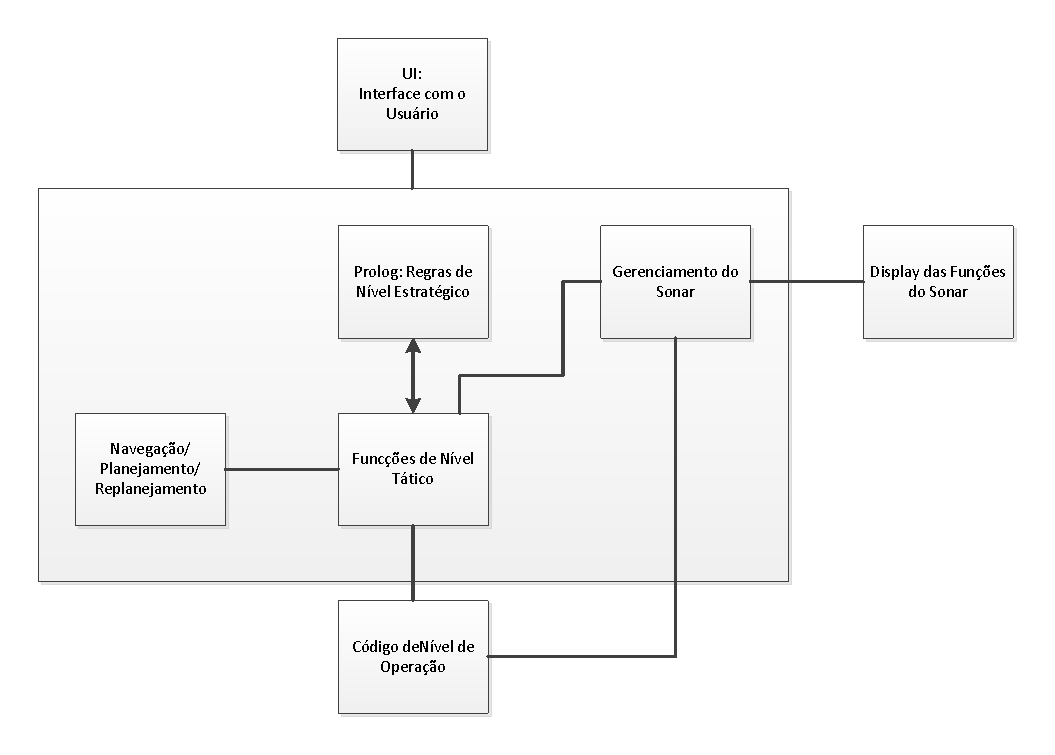
\includegraphics[width=1\columnwidth]{figs/HEALEY_1.pdf}
\caption{Arquitetura do Robô Phoenix de Healey}
\label{HEALEY_1}
\end{figure}

A terminologia de Healey, essencial para os trabalhos futuros em controle de
missão, é apresentada a seguir. Assumindo o conjunto de todos os atuadores
disponíveis no veículo como $A$, o conjunto de sensores como $S$ e o conjunto de estados
contínuos como $X$:

\textbf{Definição}: Uma Função de Controle (CF) é o uso de um subconjunto
específico de atuadores $a_i \subset A$ com um subconjunto particular de
sensores $s_i \subset S$ para estimar um subconjunto de estados contínuos $x_i
\subset X$ e levar um certo subconjunto de erros $e_i$ para zero. Onde erro é
definido como a diferença entre um valor de comando (\emph{Set Point}) e um
estado atual estimado. A definição é análoga com a definição de Tarefa do Robô
(\emph{Robot Task}), em Espiau, B. [9] (INRIA, França).

\textbf{Definição}: Primitiva de Veículo é uma \emph{string} na linguagem de
programação, associada a uma Função de Controle. Por exemplo,
$Forward_Speed_Control$, controle de velocidade do veículo.

\textbf{Definição}: O Término de uma função de controle ocorre nas seguintes
condições:
\begin{itemize}
  \item Em um tempo especificado;
  \item Quando a função positiva definida do erro, $P(\cdot)$, assume valores
  limites especificados. Quando $b$ é um limite positivo e $F(\cdot)$ é um
  filtro passa-baixa, a Terminação ocorre se
  $$F(P(e)) < b$$
\end{itemize}  
\textbf{Definição}: Um Comportamento (B) é descrito como a execução de uma
sequência particular de CFs, cada uma com sua terminação. O estado de realizar
uma certa CF é um estado discreto do sistema. Um Comportamento pode ser
representado como uma rede de Petri, por exemplo.

\textbf{Definição}: Um Sistema de Controle Híbrido é um sistema de controle de
elementos de hardware e software capaz de conduzir o veículo por um conjunto de
Comportamentos.

\textbf{Definição}: Um Plano de Missão é a sequência de Comportamentos
conduzidos durante cada fase da missão, com tratamento de falhas.

Healey define diversas Primitivas de Veículo para AUVs, mas serão estudadas as
Primitivas do Robô MARIUS, de Silva, V., que é semelhante ao robô DORIS,
objeto de estudo desta dissertação.

Em 1996, Silva, V. et al [6] (Institute for Systems and Robotics, Lisboa),
projetaram, desenvolveram e testaram um sistema de controle de missão para o
MARIUS, robô autônomo submarino. \emph{A Mission Control System} (MCS), o
conceito, aparece pela primeira vez na nomenclatura como um sistema que:
\emph{i)} habilita o operador a definir uma missão ao veículo em uma linguagem
de alto nível, que será traduzida em um plano de missão; \emph{ii)} provê
ferramentas adequadas para converter um plano de missão em um programa de
missão que pode ser verificado e executado em tempo real; \emph{iii)} fornece
ao operador a capacidade de seguir o progresso do programa de missão enquanto
ele é executado, e modificá-lo se necessário;

O trabalho de Silva, V. [6], introduz novos e importantes conceitos chave para o
MCS: Tarefa do Sistema (\emph{System Task}), Primitiva do
Veículo (\emph{Vechicle Primitive}), Procedimento de Missão (\emph{Mission Procedure})
e Programa de Missão (\emph{Mission Program}). Além disso, a arquitetura do
veículo, por ser um AUV, possui sistemas e interconexões
semelhantes ao robô DORIS, estudo desta dissertação.

A arquitetura do veículo DORIS teve grande influência da organização do veículo
MARIUS descrita abaixo, figura~\ref{SILVA_1}:
\begin{itemize}
  \item \emph{Vehicle Support System} (VSS) - Controla a distribuição de energia
  aos hardwares instalados no veículo, monitora consumo de energia e detecta
  falhas de hardware, podendo enviar comandos de emergência.
  \item \emph{Actuator Control System} (ACS) - Controla a velocidade de rotação
  dos propulsores e posição dos ailerions e lemes. Os \emph{Set Points} dos
  atuadores são dados pelo \emph{Vehicle Guidance and Control System} (VGCS) e
  os dados dos atuadores são transmitidos para o \emph{Mission Control System}.
  \item \emph{Navigation System} (NS) - Estima posição linear e velocidade do
  veículo, orientação e velocidade angular. O sistema funde informações do
  \emph{Positioning System} (\emph{Long Baseline unit}) e \emph{Motion Sensor
  Integration System}, o qual inclui diversos sensores. As saídas do NS são
  entradas do VGCS, e enviadas ao MCS.
  \item \emph{Vehicle Guidance and Control System} (VGCS) - Recebe como entrada
  as trajetórias de referência pelo MCS, e os dados de navegação do NS. Suas
  saídas são \emph{Set Points} para velocidade de rotação e outros atuadores do
  ACS, tal que o veículo siga a trajetória desejada mesmo com incertezas e
  distúrbios.
  \item \emph{Communication System} (COMS) - Controla o link bidirecional usado
  pelo operador para passar missões ao MCS, e pelo veículo para passar status de
  missão ou estados do veículo.
  \item \emph{Environmental Inspection System} (EIS) - Coleta dados do ambiente
  com diversos sensores (inclusive câmeras), como temperatura, pressão, pH. É
  controlado pelo MCS.
  \item \emph{Data Logging System} (DLS) - Adquiri e armazena dados do veículo.
  \item \emph{Mission Control System} (MCS) - Sequencia e sincroniza a execução
  das tarefas básicas do veículo para uma determinada missão e provê a
  recuperação em caso de falhas.
\end{itemize}

\begin{figure}[H]
\centering
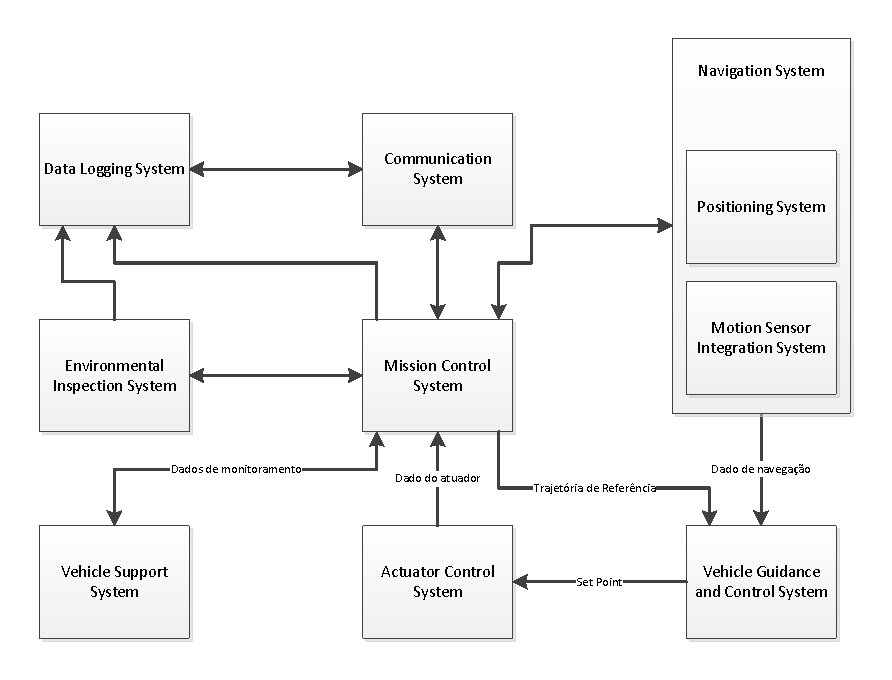
\includegraphics[width=1\columnwidth]{figs/SILVA_1.pdf}
\caption{Arquitetura do Veículo MARIUS}
\label{SILVA_1}
\end{figure}

A seguir, serão apresentados os conceitos chave de Silva, inpirados nos
trabalhos de Espiau e Healey:\\

\textbf{Tarefa do Sistema} (ST): é a especificação paramétrica de uma classe
de algoritmos ou processos que implementam uma funcionalidade básica em um robô.
Reque a implementação de dois módulos: \textit{i}) um \emph{módulo Funcional}
que contém um determinado algoritmo e precesso, e transfere dados com outras
Tarefas do Sistema e dispositivos físicos; \textit{ii}) um \emph{módulo
Comando}, máquina de estado finito, que recebe comandos externos, produz
mensagens de saída, e controla a seleção de algoritmos, processos, e caminhos
dos dados para/de módulos Funcionais.

Na modelagem do sistema em redes de Petri, quando uma transição é
disparada, uma ST é executada, chamada através do seguinte cabeçalho:
$STname(D_{mode},Din_{st},P_m)$, onde $STname$ é o nome da ST, $D_{mode}$ é uma
string de dados de entrada que especifica um determinado algoritmo ou processo a
ser executado, e $Din_{st}$ é um conjunto de dados numéricos que são entrada
desses algoritmos ou processos. $P_m$ é um parâmetro para associar ST com
Primitivas do Veículo (descritos abaixo), indicando um número finito de lugares
na rede de Petri que devem ser marcados de acordo com o tipo da saída das
mensagens das STs.

As STs do MARIUS são semelhantes aos blocos da organização do veículo,
figura~\ref{SILVA_2}:
\emph{Vehicle Support Task} (VST), \emph{Actuator Control Task} (ACT),
\emph{Vehicle Navigation Task} (VNT), \emph{Motion Sensor Task} (MST),
\emph{Guidance and Control Task} (GCT), \emph{Vehicle Communications Task}
(VCT), \emph{Space and Time Task} (STT), \emph{Vehicle Log Taks} (VLT). 

\begin{figure}[H]
\centering
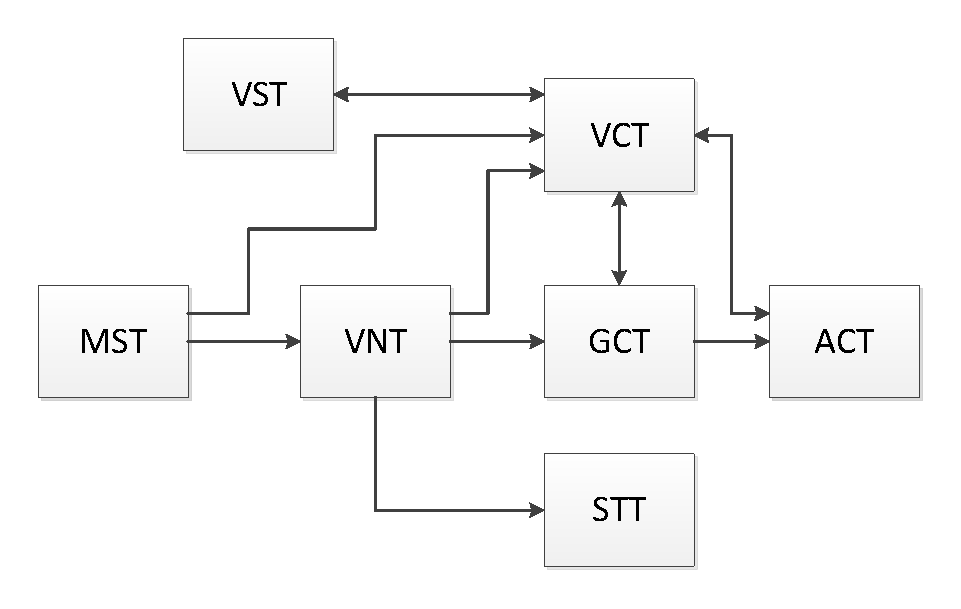
\includegraphics[width=1\columnwidth]{figs/SILVA_2.pdf}
\caption{Tarefas de Sistema do veículo MARIUS}
\label{SILVA_2}
\end{figure}

O exemplo de um cabeçalho que chama uma ST seria:
$GCT(YAW\_AUTO,\psi,p_{yaw\_auto})$, onde $GCT$ é o nome da ST, $YAW\_AUTO$
seleciona um modo de operação particular que implementa um controle automático
para guinada (\emph{yaw}), e $\psi$ é ângulo \emph{set-Point}.

\textbf{Primitiva do Veículo} (VP): é a especificação paramétrica de um modo
de operação elementar em um robô. Corresponde a ativação lógica e sincronizada
de um número de STs, as quais conduzem a um comportamento lógico e estrututrado
do veículo. Existe um conjunto de pré-condições, recursos alocados, exceções e
pós-condições associados às VPs, assim como as RT (Robot-Task) definidas em
Espiau.

A rede de Petri associada à VP é uma tupla de 5 parâmetros
$(P_{VP},T_{VP},A_{VP},\omega_{VP},X_{VP})$, onde $P_{VP},T_{VP}$ e $A_{VP}$ são
os conjuntos de lugares, transições e arcos, respectivamente, $\omega_{VP}$ é
uma função peso, e $X_{VP_{0}}$ é a condição inicial da rede de Petri. O
conjunto dos lugares pode ser decomposto em $P_{VP}=P_{pre}\cup P_{res}\cup
P_{err}\cup P_{loc}\cup P{pos}$, onde $P_{pre}$, $P_{res}$, $P_{err}$,
$P_{loc}$ e $P{pos}$ denotam os subconjuntos de lugares das pré-condições,
recursos alocados, erros, pós-condições, e os outros estados da rede de Petri,
respectivamente.

A transição em um Processo de Missão (descrito abaixo) inicializa a execução de
uma VP, chamada com o seguinte cabeçalho: $VPname(Din_{vp},P_m)$, onde
$Din_{vp}$ é o conjunto de dados numéricos que são entrada da VP e $P_m$ é o
parâmetro que associa a VP ao Processo de Missão.

\textbf{Processo de Missão} (MP): é a especificação paramétrica de uma Ação de
um sistema robótico. MP corresponde à cadeia lógica e temporal de VPs e,
possivelmente, outras MPs, as quais, em conjunto, executam uma determinada Ação.

A modelagem de MPs também pode ser em redes de Petri e é semelhante à VP, porém
em maior alto nível. O cabeçalho é: $MPname(Din_{mp},P_m)$, onde
$Din_{mp}$ é o conjunto de dados numéricos que são entrada do MP e $P_m$ é
similar à VP.

As VPs e MPs apresentadas por Silva, em [6], serão abordadas ao longo desta
dissertação de metrado, por ter grande semelhança às características do robô
DORIS, apesar de ter como enfoque AUVs. A fim de exemplificar todo o formalismo
apresentado, a modelagem da VP
$KeepHeading(\psi,p_{\textrm{Exit}},p_{\textrm{End}})$ será avaliada. A
VP é responsável por levar o robô a um determinado \emph{Set-Point} ($\psi$),
$p_{\textrm{Exit}}$ é um lugar na rede de Petri que deve ser marcado como parada
da execução da VP e $p_{\textrm{End}}$ é um lugar que tem a informação de
término da execução da VP. A única pré-condição para a execução da VP é a
inicialização de todas as ST: comando
$Init(p_{\textrm{End}},p_{\textrm{Abort}})$. Não há pós-condições e o recurso
alocado para a VP é o leme: $P_{\textrm{pre}}=\{p_{\textrm{Init}}\}$, e
$P_{res}=\{p_{\textrm{Rudder}}\}$.
A rede de Petri da VP pode ser vista na figura~\ref{SILVA_3}.

\begin{figure}[H]
\centering
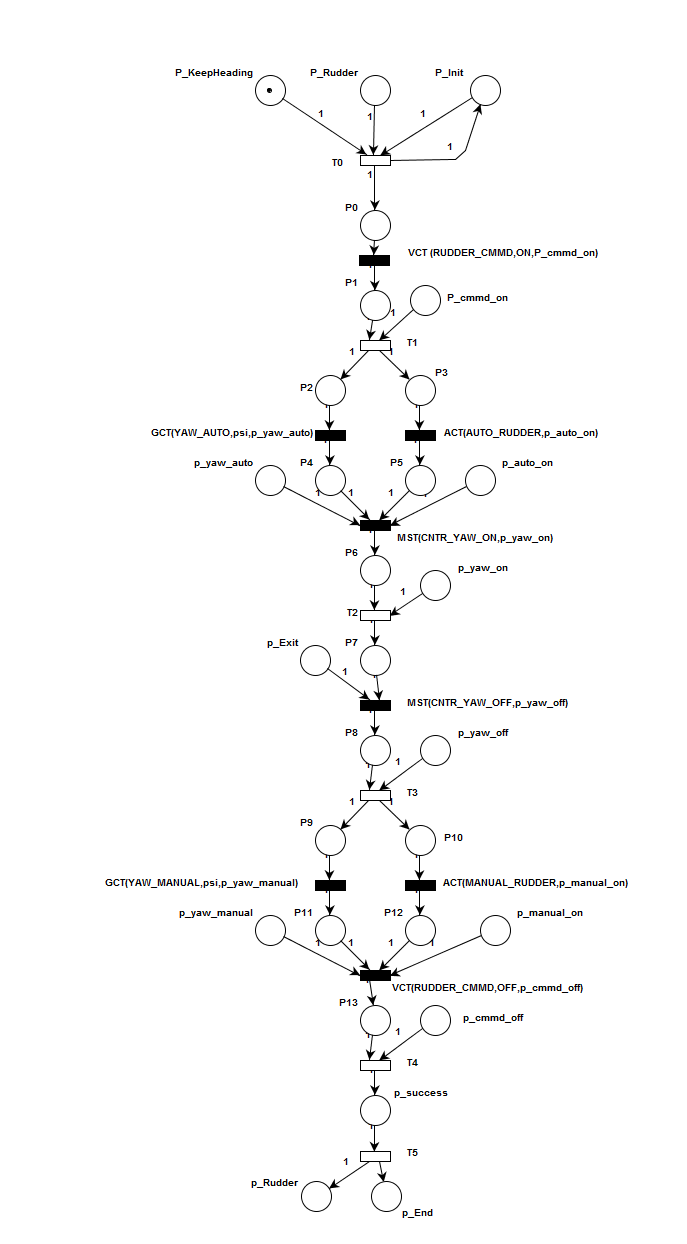
\includegraphics[width=0.87\columnwidth]{figs/SILVA_3.png}
\caption{Rede de Petri da Primitiva de Veículo KeepHeading do robô MARIUS}
\label{SILVA_3}
\end{figure}

O estado inicial da rede de Petri é: $$M
=\{1,0,0,0,0,0,0,0,0,0,0,0,0,0,0,0,0,0,0,0,0,0,0,0,0,0,0,0,0\}$$, cujos lugares
são:
$$M
=\{P_{\textrm{KeepHeading}},P_{\textrm{Rudder}},P_{\textrm{Init}},P_0,P_1,P_{\textrm{cmmd\_on}},P_2,P_3,P_{\textrm{yaw\_auto}},P_4,P_5,P_{\textrm{auto\_on}},\ldots$$
$$P_6,P_{\textrm{yaw\_on}},P_{\textrm{Exit}},P_7,P_8,P_{\textrm{yaw\_off}},P_9,P{10},P_{\textrm{yaw\_manual}},P_{11},P_{12},P_{\textrm{manual\_on}},\ldots$$
$$P_{13},P_{\textrm{cmmd\_off}},P_{\textrm{success}},P_{\textrm{Rudder}},P_{\textrm{End}}\}$$

As suas transições são:
\begin{enumerate}
  \item A transição $T0$ só pode ser disparada quando o recurso leme fica
  disponível e as ST são inicializadas:
 $$M
=\{1,1,1,0,0,0,0,0,0,0,0,0,0,0,0,0,0,0,0,0,0,0,0,0,0,0,0,0,0\}$$
Após a transição $T0$:
  $$M
=\{0,0,0,1,0,0,0,0,0,0,0,0,0,0,0,0,0,0,0,0,0,0,0,0,0,0,0,0,0\}$$  
  \item A transição $VCT(RUDDER\_CMMD,ON,P_{\textrm{cmmd\_on}})$
  (\emph{Vehicle Communications Task}) é ST para desabilitar comandos diretos ao
  leme do console (operador).
$$M
=\{0,0,0,0,1,0,0,0,0,0,0,0,0,0,0,0,0,0,0,0,0,0,0,0,0,0,0,0,0\}$$ 
  \item A transição $T1$ é habilitada após a alteração da ST VCT for concluída
  e $P_{\textrm{cmmd\_on}}$ for marcada (token). $$M
=\{0,0,0,0,1,1,0,0,0,0,0,0,0,0,0,0,0,0,0,0,0,0,0,0,0,0,0,0,0\}$$
Após a transição $T1$:
$$M
=\{0,0,0,0,0,0,1,1,0,0,0,0,0,0,0,0,0,0,0,0,0,0,0,0,0,0,0,0,0\}$$
  \item As transições $ACT(AUTO\_RUDDER,P_{\textrm{auto\_on}})$
  (\emph{Actuator Control Task}) e $GCT(YAW\_AUTO,\Psi,P_{\textrm{yaw\_auto}})$
  (\emph{Guidance and Control Task}) são ativadas paralelamente. A primeira está
  associada à ST para habilitar o leme a receber comandos diretamente do
  controlador. A ST GCT é requisitada para ativar o controle de guinada
  (\emph{Yaw}) e recebe como argumento o \emph{set-point} $\psi$.
$$M
=\{0,0,0,0,0,0,0,0,0,1,1,0,0,0,0,0,0,0,0,0,0,0,0,0,0,0,0,0,0\}$$
  \item A transição $MST(CNTR\_YAW\_ON,P_{\textrm{yaw\_on}})$ (\emph{Motion
  Sensor Task}) é habilitada após as alterações das STs ACT e GCT serem
  concluídas.
  $P_{\textrm{yaw\_auto}}$ e $P_{\textrm{autoon}}$ são marcados (tokens):
  $$M
=\{0,0,0,0,0,0,0,0,1,1,1,1,0,0,0,0,0,0,0,0,0,0,0,0,0,0,0,0,0\}$$
A ST MST é chamada para enviar dados dos sensores de ângulo de guinada
periodicamente para a ST GCT.
Após a transição
$MST(CNTR\_YAW\_ON,P_{\textrm{yaw\_on}})$:
  $$M
=\{0,0,0,0,0,0,0,0,0,0,0,0,1,0,0,0,0,0,0,0,0,0,0,0,0,0,0,0,0\}$$
  \item A transição $T2$ só é habilitada quando a alteração da ST MST for
  concluída e, assim, $P_{\textrm{yaw\_on}}$ adquire um token:
    $$M
=\{0,0,0,0,0,0,0,0,0,0,0,0,1,1,0,0,0,0,0,0,0,0,0,0,0,0,0,0,0\}$$
Após transição de $T2$:
$$M
=\{0,0,0,0,0,0,0,0,0,0,0,0,0,0,0,1,0,0,0,0,0,0,0,0,0,0,0,0,0\}$$
  \item Em $P_7$, o robô permanece em sistema de controle em malha fechada da VP
  KeepHeading até que o lugar $P_{\textrm{Exit}}$ seja marcado:
$$M
=\{0,0,0,0,0,0,0,0,0,0,0,0,0,0,1,1,0,0,0,0,0,0,0,0,0,0,0,0,0\}$$
A transição $MST(CNTR\_YAW\_OFF,P_{\textrm{yaw\_off}})$ é, então, habilitada. A
ST MST é, novamente, chamada para desabilitar o envio de mensagens à GCT. Após a
transição da $MST(CNTR\_YAW\_OFF,P_{\textrm{yaw\_off}})$:
$$M
=\{0,0,0,0,0,0,0,0,0,0,0,0,0,0,0,0,1,0,0,0,0,0,0,0,0,0,0,0,0\}$$
  \item As transições $T3$, $GCT(YAW\_MANUAL,P_{\textrm{yaw\_manual}})$,
  $ACT(MANUAL\_RUDDER,P_{\textrm{manual\_on}})$ e
  $VCT(RUDDER\_CMMD,OFF,P_{\textrm{cmmd\_off}})$ alteram as STs GCT, ACT e VCT
  para levarem ao estados manual, como era inicialmente. Os estados para isso
  são:
$$M
=\{0,0,0,0,0,0,0,0,0,0,0,0,0,0,0,0,1,1,0,0,0,0,0,0,0,0,0,0,0\}$$
$$M
=\{0,0,0,0,0,0,0,0,0,0,0,0,0,0,0,0,0,0,1,1,0,0,0,0,0,0,0,0,0\}$$
$$M
=\{0,0,0,0,0,0,0,0,0,0,0,0,0,0,0,0,0,0,0,0,0,1,1,0,0,0,0,0,0\}$$
$$M
=\{0,0,0,0,0,0,0,0,0,0,0,0,0,0,0,0,0,0,0,0,1,1,1,1,0,0,0,0,0\}$$
$$M
=\{0,0,0,0,0,0,0,0,0,0,0,0,0,0,0,0,0,0,0,0,0,0,0,0,1,0,0,0,0\}$$
$$M
=\{0,0,0,0,0,0,0,0,0,0,0,0,0,0,0,0,0,0,0,0,0,0,0,0,1,1,0,0,0\}$$
$$M
=\{0,0,0,0,0,0,0,0,0,0,0,0,0,0,0,0,0,0,0,0,0,0,0,0,0,0,1,0,0\}$$  
  \item A última transição $T5$ libera o recurso $P_{\textrm{Rudder}}$ e
  finaliza a VP no lugar $P_{\textrm{End}}$:
$$M
=\{0,0,0,0,0,0,0,0,0,0,0,0,0,0,0,0,0,0,0,0,0,0,0,0,0,0,0,1,1\}$$
\end{enumerate} 

Silva desenvolveu os softwares CORAL e ATOL para implementação das VPs e STs em
redes de Petri de forma que um usuário final, como um operador, pudesse
facilmente criar seus MPs. A grande contribuição 



